% 2D Rotation Coordinates
%
% File:         2d-rotation-coordinates.tex
% Author:       Bob Walton (walton@acm.org)
% Date:      	Fri Dec 21 05:46:58 EST 2012
  
\documentclass{minimal}
\usepackage[paperheight=2.4in,paperwidth=2.8in,
            height=2.4in,hoffset=0.2in,
	    voffset=0.05in,left=0in,width=2.8in]{geometry}
\usepackage{color}
\usepackage[usenames]{xcolor}
\usepackage{scalefnt}
\usepackage[greek,english]{babel}
\usepackage{tikz}
\newcommand{\SMALL}{\scalefont{0.8}}
\newcommand{\THETA}{{\greektext J}}
\usetikzlibrary{arrows}
\begin{document}
\raggedright
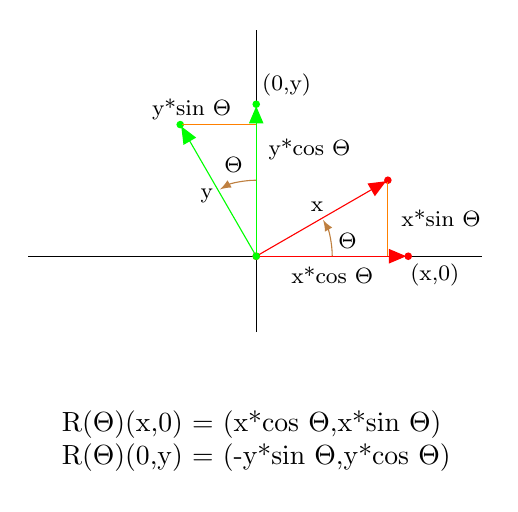
\begin{tikzpicture}[x=0.190in,y=0.190in]
\begin{scope}[yshift=1in,>=triangle 45,shorten >=0.01in]
    \draw[black] (-6,0) -- (+6,0);
    \draw[black] (0,-2) -- (0,+6);

    \fill[red] (0,0) circle(0.1) (4,0) circle(0.1);
    \draw[red,->] (0,0) -- (4,0);
    \draw[black] (4.7,-0.5) node{\SMALL (x,0)};
    \draw[black] (2.0,-0.5) node{\SMALL x*cos \THETA};

    \draw[brown,>=latex,->] (2.0,0) arc(0:30:2.0);
    \draw[black] (2.4,+0.4) node{\SMALL \THETA};

    \fill[red] (3.464101615,2.0) circle(0.1);
    \draw[red,->] (0,0) -- (3.464101615,2.0);
    \draw[black] (1.6,+1.3) node{\SMALL x};

    \draw[orange] (3.464101615,0) -- (3.464101615,2.0);
    \draw[black] (3.464101615,1) + (0.1,0) node[right]{\SMALL x*sin \THETA};

    \fill[green] (0,0) circle(0.1) (0,4) circle(0.1);
    \draw[green,->] (0,0) -- (0,4);
    \draw[black] (0.8,4.5) node{\SMALL (0,y)};
    \draw[black] (1.4,2.8) node{\SMALL y*cos \THETA};

    \draw[brown,>=latex,->] (0,2.0) arc(90:120:2.0);
    \draw[black] (-0.6,2.4) node{\SMALL \THETA};

    \fill[green] (-2.0,3.464101615) circle(0.1);
    \draw[green,->] (0,0) -- (-2.0,3.464101615);
    \draw[black] (-1.3,1.6) node{\SMALL y};

    \draw[orange] (0,3.464101615) -- (-2.0,3.464101615);
    \draw[black] (-1.0,3.464101615) + (-2.0,0.4) node[right]{\SMALL y*sin \THETA};
\end{scope}

\begin{scope}
\draw (0,0.4) node {
    $\begin{tabular}[t]{l}
    R(\THETA)(x,0) = (x*cos \THETA,x*sin \THETA) \\
    R(\THETA)(0,y) = (-y*sin \THETA,y*cos \THETA) \\
    \end{tabular}$
    };
\end{scope}
\end{tikzpicture}
\end{document}



